\documentclass[final,t]{beamer}

\usepackage[orientation=landscape,size=custom,width=91.44,height=60.96,scale=1.15]{beamerposter}

\usepackage{lmodern}
\usepackage[T1]{fontenc}
\usepackage{helvet}
\renewcommand{\familydefault}{\sfdefault}

\usepackage{graphicx}
\usepackage{booktabs}
\usepackage{xcolor}
\usepackage{tikz}
\usepackage{amsmath,amssymb}
\usepackage{enumitem}
\usepackage{adjustbox}
\usepackage[most]{tcolorbox}

\usetikzlibrary{positioning, arrows.meta, backgrounds, calc, shadows, shapes.geometric, fit}

\definecolor{cornellred}{HTML}{B31B1B}
\definecolor{bodygray}{HTML}{222222}
\definecolor{lightgray}{HTML}{F2F2F2}
\definecolor{boxbg}{HTML}{F9F9F9}

\setbeamercolor{background canvas}{bg=white}
\setbeamercolor{structure}{fg=cornellred}
\setbeamercolor{normal text}{fg=bodygray}

\setbeamertemplate{navigation symbols}{}
\setbeamertemplate{caption}[numbered]
\setbeamerfont{caption}{size=\small}

\newlength{\colw}
\setlength{\colw}{0.188\paperwidth}
\newlength{\colsep}
\setlength{\colsep}{0.01\paperwidth}

\tcbset{
  posterbox/.style={
    enhanced,
    colback=boxbg,
    colframe=cornellred,
    boxrule=1.5pt,
    arc=4mm,
    auto outer arc,
    coltitle=white,
    fonttitle=\large\bfseries,
    toptitle=3mm,
    bottomtitle=3mm,
    titlerule=0pt,
    drop fuzzy shadow,
    boxsep=2mm,
    left=3mm,
    right=3mm,
    top=2mm,
    bottom=2mm,
    equal height group=cols,
  }
}

\begin{document}

\begin{frame}[fragile]

\begin{tikzpicture}[remember picture, overlay]
  \fill[cornellred]
    ($(current page.north west)$) rectangle
    ($(current page.north east)+(0,-0.115\paperheight)$);

  \node[anchor=west, xshift=0.015\paperwidth, yshift=-0.058\paperheight,
        text=white, align=left] at (current page.north west) {%
    \fontsize{28}{34}\selectfont\bfseries Cornell University\\
    \fontsize{18}{22}\selectfont CS 4782 \textperiodcentered{} Spring 2026};

  \node[anchor=center, yshift=-0.058\paperheight, text=white, align=center]
    at (current page.north) {%
    \fontsize{56}{64}\selectfont\bfseries Many Heads Are Better Than One\\[1.5ex]
    \fontsize{30}{36}\selectfont\mdseries Reproducing MEDUSA
    \textendash{} Speculative Decoding with Four Drafting Heads on Vicuna-7B};

  \node[anchor=east, xshift=-0.015\paperwidth, yshift=-0.058\paperheight,
        text=white, align=right] at (current page.north east) {%
    \fontsize{24}{28}\selectfont\bfseries Huajie Zhong \textperiodcentered{} Frank Dai\\
    \fontsize{18}{22}\selectfont\mdseries hz642 \textperiodcentered{} sd924};
\end{tikzpicture}

\vspace{0.12\paperheight}

\centering
\begin{minipage}{0.97\paperwidth}

% Column 1
\begin{minipage}[t]{\colw}\setlength{\parskip}{0.5ex}\raggedright\vspace{0pt}

\begin{tcolorbox}[posterbox, title=1. Motivation]
\textbf{The problem.} LLM inference is bottlenecked by \emph{sequential} token generation: one token per forward pass. At batch size 1, GPUs are \emph{memory-bandwidth-bound}, not compute-bound --- most of the silicon is idle every step.

\textbf{The goal.} Generate multiple tokens per forward pass \emph{without} sacrificing output quality.

\textbf{MEDUSA} [Cai et al., 2024] attaches $K$ extra decoding heads to a frozen backbone, predicting tokens $k$ steps ahead in parallel. A tree-attention \emph{verification} pass checks all candidate continuations at once, and an acceptance rule guarantees quality.

\vspace{0.5ex}
\textbf{Paper target (\S3.1):}\\ MEDUSA-1 on Vicuna-7B $\to$ \textbf{2.18$\times$} speedup.

\vspace{0.8ex}
\centering
\fbox{\begin{minipage}{0.93\colw}\centering
\textit{[Optional funny image:\\ assets/funny\_medusa.png]}\\[0.5ex]
\scriptsize (drop in before final build)
\end{minipage}}
\end{tcolorbox}

\end{minipage}%
\hspace{\colsep}%
% Column 2
\begin{minipage}[t]{\colw}\setlength{\parskip}{0.5ex}\raggedright\vspace{0pt}

\begin{tcolorbox}[posterbox, title=2. Architecture]
\textbf{MedusaHead:} two-layer residual block
\[ y = W_2\bigl(\mathrm{SiLU}(W_1 h) + h\bigr) \]
\textbf{Key init trick:} $W_1 \!=\! 0$, $W_2 \!=\! $ \texttt{lm\_head.clone()}.\\
At step 0 each head \emph{exactly} reproduces the original distribution --- stable starting point.

\vspace{0.4ex}
\centering
\begin{tikzpicture}[font=\small,
    headnode/.style={draw=cornellred, rounded corners=3pt, fill=cornellred!10, minimum width=7cm, minimum height=0.9cm, drop shadow, font=\bfseries},
    hnode/.style={draw=gray, rounded corners=3pt, fill=gray!15, minimum width=7cm, minimum height=1.0cm, drop shadow, font=\bfseries}]
  \node[hnode] (h) at (0,0) {Hidden states $h$};
  \node[headnode] (lm) at (0,-1.9) {LM head $\to$ token $t{+}1$};
  \node[headnode] (h0) at (0,-3.2) {Head 0 $\to$ $t{+}2$};
  \node[headnode] (h1) at (0,-4.5) {Head 1 $\to$ $t{+}3$};
  \node[headnode] (h2) at (0,-5.8) {Head 2 $\to$ $t{+}4$};
  \node[headnode] (h3) at (0,-7.1) {Head 3 $\to$ $t{+}5$};
  \draw[-{Latex[length=3mm]}, thick, cornellred] (h) -- (lm);
  
  \draw[thick, cornellred] (h.west) -- ++(-0.6,0) coordinate (trunk);
  \draw[-{Latex[length=3mm]}, thick, cornellred, rounded corners=4pt] (trunk) |- (h0.west);
  \draw[-{Latex[length=3mm]}, thick, cornellred, rounded corners=4pt] (trunk) |- (h1.west);
  \draw[-{Latex[length=3mm]}, thick, cornellred, rounded corners=4pt] (trunk) |- (h2.west);
  \draw[-{Latex[length=3mm]}, thick, cornellred, rounded corners=4pt] (trunk) |- (h3.west);
\end{tikzpicture}

\raggedright
\vspace{0.3ex}
\textbf{Training (MEDUSA-1, frozen backbone):}\\
$K{=}4$ heads only \textperiodcentered{} loss $\mathcal{L}=\sum_{k=1}^{K} 0.8^{k}\mathcal{L}_k$ \textperiodcentered{} 60k ShareGPT samples \textperiodcentered{} AdamW $10^{-3}$ \textperiodcentered{} H100 bf16.
\end{tcolorbox}

\end{minipage}%
\hspace{\colsep}%
% Column 3
\begin{minipage}[t]{\colw}\setlength{\parskip}{0.5ex}\raggedright\vspace{0pt}

\begin{tcolorbox}[posterbox, title=3. Tree Attention]
One forward pass verifies \textbf{64 candidate tokens}.\\
Each node attends to \textcolor{gray!70!black}{prefix} + \textcolor{cornellred}{ancestors} only --- not siblings, not cousins.

\vspace{0.4ex}
\centering
\begin{tikzpicture}[font=\small,
    cnode/.style={draw=darkgray, circle, minimum size=1.1cm, fill=gray!20, drop shadow},
    rnode/.style={draw=cornellred!80!black, circle, minimum size=1.1cm, fill=cornellred, text=white, drop shadow, font=\bfseries},
    anode/.style={draw=cornellred!80!black, circle, minimum size=1.1cm, fill=cornellred!40, drop shadow},
    cnode_highlight/.style={draw=cornellred!80!black, circle, minimum size=1.1cm, fill=cornellred!70, text=white, drop shadow, font=\bfseries}]
    
  \node[cnode] (p1) at (-4, 1.0) {$P_1$};
  \node[cnode] (p2) at (-2.5, 1.0) {$P_2$};
  \draw[dashed, thick, gray] (p1) -- (p2);

  \node[rnode] (r) at (0, 1.0) {root};
  \node[anode] (a) at (-1.2, -0.5) {A};
  \node[cnode] (b) at (1.2, -0.5) {B};
  \node[cnode_highlight] (c) at (-2.0, -2.0) {C};
  \node[cnode] (d) at (-0.4, -2.0) {D};

  \draw[thick, cornellred] (r) -- (a);
  \draw[thick, darkgray] (r) -- (b);
  \draw[thick, cornellred] (a) -- (c);
  \draw[thick, darkgray] (a) -- (d);
  \draw[-{Latex[length=3mm]}, gray, thick] (p2) -- (r);

  % Background highlight for attention path
  \begin{scope}[on background layer]
    \draw[cornellred!15, line width=1.5cm, line cap=round, line join=round] (r.center) -- (a.center) -- (c.center);
    \draw[gray!15, line width=1.5cm, line cap=round, line join=round] (p1.center) -- (p2.center);
  \end{scope}
\end{tikzpicture}

\raggedright
\vspace{0.4ex}
\textbf{Mask for C:} attends to \textcolor{gray}{prefix $(P_1,P_2)$} + \textcolor{cornellred}{ancestors (root, A)} + self; \emph{not} siblings (B, D).

\vspace{0.3ex}
\textbf{Static 64-node tree:} widths $s=[10,3,2,2]$, BFS-ordered.

\vspace{0.2ex}
\textbf{Acceptance criteria}:
\begin{itemize}[leftmargin=*, topsep=0.4ex, itemsep=0.2ex]
  \item \textbf{Greedy}: $\arg\max\!=\!$child $\Rightarrow$ bitwise-identical to autoregressive baseline.
  \item \textbf{Typical} (\S2.3.1): $p(x) > \min(\varepsilon, \delta e^{-H(p)})$, $\varepsilon\!=\!\delta\!=\!0.09$ \textendash{} distributionally equivalent to sampling from the original.
\end{itemize}
\end{tcolorbox}

\end{minipage}%
\hspace{\colsep}%
% Column 4
\begin{minipage}[t]{\colw}\setlength{\parskip}{0.5ex}\raggedright\vspace{0pt}

\begin{tcolorbox}[posterbox, title=4. Results]
\centering
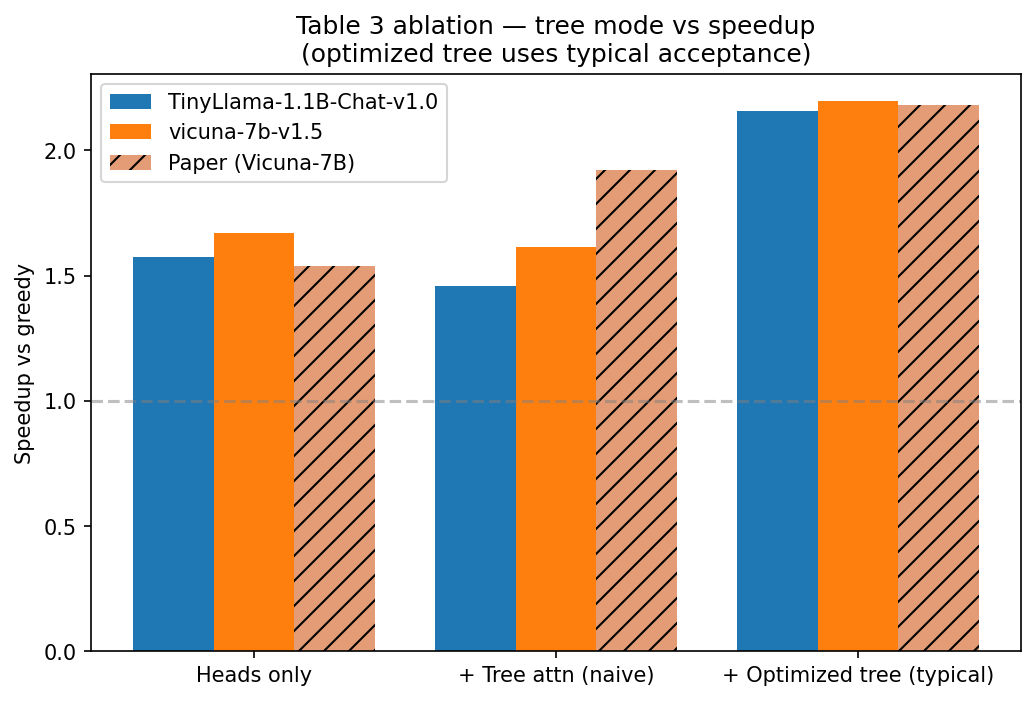
\includegraphics[width=\colw]{../results/table3_comparison.png}\\
{\scriptsize Figure 1: Table 3 ablation vs. paper targets.}

\vspace{0.5ex}
\small
\begin{tabular}{@{}lcc@{}}
\toprule
\textbf{Configuration} & \textbf{Paper} & \textbf{Ours}\\
\midrule
Heads only         & 1.54$\times$ & \textbf{1.67$\times$}\\
+ Naive tree       & 1.92$\times$ & 1.62$\times$\\
+ Opt.\ tree (greedy) & ---       & 2.034$\times$\\
+ Opt.\ tree (typical) & \textbf{2.18$\times$} & \textbf{2.196$\times$} \checkmark\\
\midrule
Head-0 accuracy    & $>$60\%     & \textbf{64.1\%}\\
Accept.\ length    & 3.47 (MED-2) & \textbf{2.87}\\
\bottomrule
\end{tabular}\\[0.6ex]
{\scriptsize Table 1: Our reproduction matches the paper's 2.18$\times$ target.}

\vspace{0.4ex}
\centering
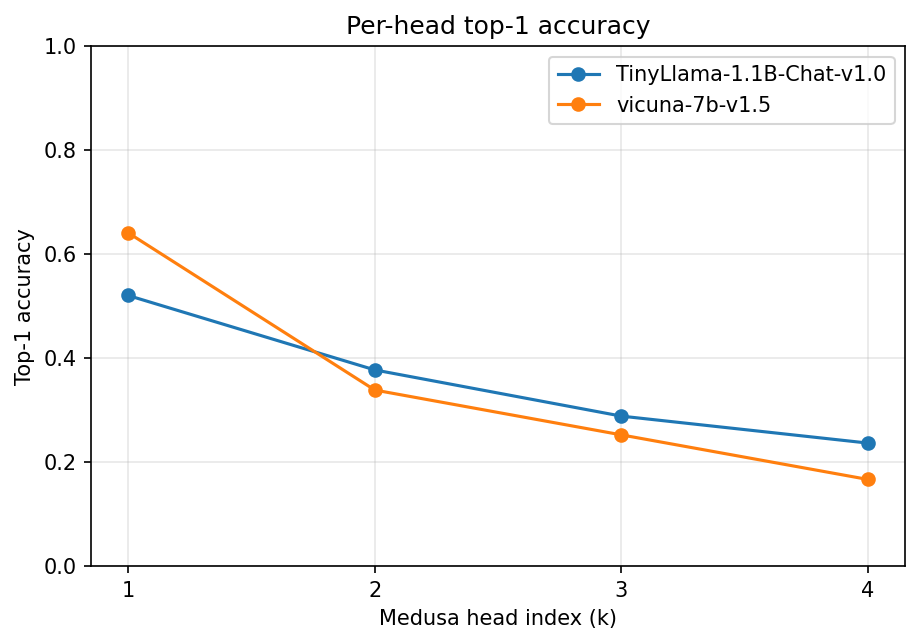
\includegraphics[width=\colw]{../results/head_accuracies.png}\\
{\scriptsize Figure 2: Per-head accuracy \textendash{} 64.1\% $\to$ 16.7\% across heads 0\textendash{}3.}
\end{tcolorbox}

\end{minipage}%
\hspace{\colsep}%
% Column 5
\begin{minipage}[t]{\colw}\setlength{\parskip}{0.5ex}\raggedright\vspace{0pt}

\begin{tcolorbox}[posterbox, title=5. Key Insight \& Takeaways]
\raggedright
\textbf{Headline result.}\\
\textbf{2.196$\times$} speedup with typical acceptance on Vicuna-7B --- matches the paper's \textbf{2.18$\times$} target.

\vspace{0.4ex}
\textbf{Surprise finding.}\\
A \emph{naive} tree (1.62$\times$) is \emph{slower} than no tree at all (1.67$\times$): a dense 64$\times$64 attention mask costs more than the $\approx$0.03 extra tokens/step it buys. Tree-structure optimization is \textbf{load-bearing}, not cosmetic.

\vspace{0.4ex}
\textbf{Typical $>$ greedy acceptance.}\\
$+18\%$ effective tokens/step (2.87 vs.\ 2.59) with the \S2.3.1 distributional-equivalence guarantee.

\vspace{0.4ex}
\textbf{Gap analysis.} Our 2.87 eff.\ tokens/step sits below MEDUSA-2's 3.47 but meets the MEDUSA-1 $<$3.0 target. Residual gap: training on raw ShareGPT rather than Vicuna-regenerated responses.

\vspace{0.4ex}
\textbf{Future work.}
\begin{itemize}[leftmargin=*, topsep=0.2ex, itemsep=0.1ex]
  \item MEDUSA-2: joint fine-tuning with self-distillation (paper target $\sim$2.8$\times$).
  \item Regenerate training data from Vicuna-7B itself.
\end{itemize}

\vspace{0.4ex}
\hrule
\vspace{0.3ex}
\begin{minipage}[t]{0.65\colw}
{\tiny
\textbf{References}\\
{[1]} Cai et al. MEDUSA. arXiv:2401.10774 (2024).\\
{[2]} Touvron et al. Llama 2. arXiv:2307.09288 (2023).\\
{[3]} Wolf et al. Transformers. EMNLP Demos (2020).\\
{[4]} Aeala. ShareGPT\_Vicuna\_unfiltered.
}
\end{minipage}\hfill
\begin{minipage}[t]{0.30\colw}\centering
\includegraphics[width=0.95\linewidth]{assets/github_qr.png}\\
{\tiny\emph{scan for code}}
\end{minipage}
\end{tcolorbox}

\end{minipage}%
\end{minipage}

\end{frame}
\end{document}
